% Lines starting with a percent sign (%) are comments. LaTeX will 
% not process those lines. Similarly, everything after a percent 
% sign in a line is considered a comment. To produce a percent sign
% in the output, write \% (backslash followed by the percent sign). 
% ==================================================================
% Usage instructions:
% ------------------------------------------------------------------
% The file is heavily commented so that you know what the various
% commands do. Feel free to remove any comments you don't need from
% your own copy. When redistributing the example thesis file, please
% retain all the comments for the benefit of other thesis writers! 
% ==================================================================
% Compilation instructions: 
% ------------------------------------------------------------------
% Use pdflatex to compile! Input images are expected as PDF files.
% Example compilation:
% ------------------------------------------------------------------
% > pdflatex thesis-example.tex
% > bibtex thesis-example
% > pdflatex thesis-example.tex
% > pdflatex thesis-example.tex
% ------------------------------------------------------------------
% You need to run pdflatex multiple times so that all the cross-references
% are fixed. pdflatex will tell you if you need to re-run it (a warning
% will be issued)  
% ------------------------------------------------------------------
% Compilation has been tested to work in ukk.cs.hut.fi and kosh.hut.fi
% - if you have problems of missing .sty -files, then the local LaTeX
% For example, when compiling in vipunen.hut.fi, you get an error that
% tikz.sty is missing - in this case you must either compile somewhere
% else, or you cannot use TikZ graphics in your thesis and must therefore
% remove or comment out the tikz package and all the tikz definitions. 
% ------------------------------------------------------------------
 
% General information
% ==================================================================
% Package documentation:
% 
% The comments often refer to package documentation. (Almost) all LaTeX
% packages have documentation accompanying them, so you can read the
% package documentation for further information. When a package 'xxx' is
% installed to your local LaTeX environment (the document compiles
% when you have \usepackage{xxx} and LaTeX does not complain), you can 
% find the documentation somewhere in the local LaTeX texmf directory
% hierarchy. In ukk.cs.hut.fi, this is /usr/texlive/2008/texmf-dist,
% and the documentation for the titlesec package (for example) can be 
% found at /usr/texlive/2008/texmf-dist/doc/latex/titlesec/titlesec.pdf.
% Most often the documentation is located as a PDF file in 
% /usr/texlive/2008/texmf-dist/doc/latex/xxx, where xxx is the package name; 
% however, documentation for TikZ is in
% /usr/texlive/2008/texmf-dist/doc/latex/generic/pgf/pgfmanual.pdf
% (this is because TikZ is a front-end for PGF, which is meant to be a 
% generic portable graphics format for LaTeX).
% You can try to look for the package manual using the ``find'' shell
% command in Linux machines; the find databases are up-to-date at least
% in ukk.cs.hut.fi. Just type ``find xxx'', where xxx is the package
% name, and you should find a documentation file.
% Note that in some packages, the documentation is in the DVI file
% format. In this case, you can copy the DVI file to your home directory,
% and convert it to PDF with the dvipdfm command (or you can read the
% DVI file directly with a DVI viewer).
% 
% If you can't find the documentation for a package, just try Googling
% for ``latex packagename''; most often you can get a direct link to the
% package manual in PDF format.
% ------------------------------------------------------------------


% Document class for the thesis is report
% ------------------------------------------------------------------
% You can change this but do so at your own risk - it may break other things.
% Note that the option pdftext is used for pdflatex; there is no
% pdflatex option. 
% ------------------------------------------------------------------
\documentclass[12pt,a4paper,oneside,pdftex]{report}

% The input files (tex files) are encoded with the latin-1 encoding 
% (ISO-8859-1 works). Change the latin1-option if you use UTF8 
% (at some point LaTeX did not work with UTF8, but I'm not sure
% what the current situation is) 
\usepackage[latin1]{inputenc}
% OT1 font encoding seems to work better than T1. Check the rendered
% PDF file to see if the fonts are encoded properly as vectors (instead
% of rendered bitmaps). You can do this by zooming very close to any letter 
% - if the letter is shown pixelated, you should change this setting 
% (try commenting out the entire line, for example).  
\usepackage[OT1]{fontenc}
% The babel package provides hyphenating instructions for LaTeX. Give
% the languages you wish to use in your thesis as options to the babel
% package (as shown below). You can remove any language you are not
% going to use.
% Examples of valid language codes: english (or USenglish), british, 
% finnish, swedish; and so on.
\usepackage[english]{babel}


% Font selection
% ------------------------------------------------------------------
% The default LaTeX font is a very good font for rendering your 
% thesis. It is a very professional font, which will always be 
% accepted. 
% If you, however, wish to spicen up your thesis, you can try out
% these font variants by uncommenting one of the following lines
% (or by finding another font package). The fonts shown here are 
% all fonts that you could use in your thesis (not too silly). 
% Changing the font causes the layouts to shift a bit; you many
% need to manually adjust some layouts. Check the warning messages
% LaTeX gives you.
% ------------------------------------------------------------------
% To find another font, check out the font catalogue from
% http://www.tug.dk/FontCatalogue/mathfonts.html
% This link points to the list of fonts that support maths, but
% that's a fairly important point for master's theses.
% ------------------------------------------------------------------
% <rant>
% Remember, there is no excuse to use Comic Sans, ever, in any
% situation! (Well, maybe in speech bubbles in comics, but there 
% are better options for those too)
% </rant>

% \usepackage{palatino}
% \usepackage{tgpagella}



% Optional packages
% ------------------------------------------------------------------
% Select those packages that you need for your thesis. You may delete
% or comment the rest.

% Natbib allows you to select the format of the bibliography references.
% The first example uses numbered citations: 
\usepackage[square,sort&compress,numbers]{natbib}
% The second example uses author-year citations.
% If you use author-year citations, change the bibliography style (below); 
% acm style does not work with author-year citations.
% Also, you should use \citet (cite in text) when you wish to refer
% to the author directly (\citet{blaablaa} said blaa blaa), and 
% \citep when you wish to refer similarly than with numbered citations
% (It has been said that blaa blaa~\citep{blaablaa}).
% \usepackage[square]{natbib}

% The alltt package provides an all-teletype environment that acts
% like verbatim but you can use LaTeX commands in it. Uncomment if 
% you want to use this environment. 
% \usepackage{alltt}

% The eurosym package provides a euro symbol. Use with \euro{}
\usepackage{eurosym} 

% Verbatim provides a standard teletype environment that renderes
% the text exactly as written in the tex file. Useful for code
% snippets (although you can also use the listings package to get
% automatic code formatting). 
\usepackage{verbatim}

% The listing package provides automatic code formatting utilities
% so that you can copy-paste code examples and have them rendered
% nicely. See the package documentation for details.
% \usepackage{listings}

% The fancuvrb package provides fancier verbatim environments 
% (you can, for example, put borders around the verbatim text area
% and so on). See package for details.
% \usepackage{fancyvrb}

% Supertabular provides a tabular environment that can span multiple 
% pages. 
%\usepackage{supertabular}
% Longtable provides a tabular environment that can span multiple 
% pages. This is used in the example acronyms file. 
\usepackage{longtable}

% The fancyhdr package allows you to set your the page headers 
% manually, and allows you to add separator lines and so on. 
% Check the package documentation. 
% \usepackage{fancyhdr}

% Subfigure package allows you to use subfigures (i.e. many subfigures
% within one figure environment). These can have different labels and
% they are numbered automatically. Check the package documentation. 
\usepackage{subfigure}

% The titlesec package can be used to alter the look of the titles 
% of sections, chapters, and so on. This example uses the ``medium'' 
% package option which sets the titles to a medium size, making them
% a bit smaller than what is the default. You can fine-tune the 
% title fonts and sizes by using the package options. See the package
% documentation.
\usepackage[medium]{titlesec}

% The TikZ package allows you to create professional technical figures.
% The learning curve is quite steep, but it is definitely worth it if 
% you wish to have really good-looking technical figures. 
\usepackage{tikz}
% You also need to specify which TikZ libraries you use
\usetikzlibrary{positioning}
\usetikzlibrary{calc}
\usetikzlibrary{arrows}
\usetikzlibrary{decorations.pathmorphing,decorations.markings}
\usetikzlibrary{shapes}
\usetikzlibrary{patterns}


% The aalto-thesis package provides typesetting instructions for the
% standard master's thesis parts (abstracts, front page, and so on)
% Load this package second-to-last, just before the hyperref package.
% Options that you can use: 
%   mydraft - renders the thesis in draft mode. 
%             Do not use for the final version. 
%   doublenumbering - [optional] number the first pages of the thesis
%                     with roman numerals (i, ii, iii, ...); and start
%                     arabic numbering (1, 2, 3, ...) only on the 
%                     first page of the first chapter
%   twoinstructors  - changes the title of instructors to plural form
%   twosupervisors  - changes the title of supervisors to plural form
%\usepackage[mydraft,twosupervisors]{aalto-thesis}
\usepackage[mydraft,doublenumbering]{aalto-thesis}
%\usepackage[mydraft]{aalto-thesis}


% Hyperref
% ------------------------------------------------------------------
% Hyperref creates links from URLs, for references, and creates a
% TOC in the PDF file.
% This package must be the last one you include, because it has
% compatibility issues with many other packages and it fixes
% those issues when it is loaded.   
\RequirePackage[pdftex]{hyperref}
% Setup hyperref so that links are clickable but do not look 
% different
\hypersetup{colorlinks=false,raiselinks=false,breaklinks=true}
\hypersetup{pdfborder={0 0 0}}
\hypersetup{bookmarksnumbered=true}
% The following line suggests the PDF reader that it should show the 
% first level of bookmarks opened in the hierarchical bookmark view. 
\hypersetup{bookmarksopen=true,bookmarksopenlevel=1}
% Hyperref can also set up the PDF metadata fields. These are
% set a bit later on, after the thesis setup.   


% Thesis setup
% ==================================================================
% Change these to fit your own thesis.
% \COMMAND always refers to the English version;
% \FCOMMAND refers to the Finnish version; and
% \SCOMMAND refers to the Swedish version.
% You may comment/remove those language variants that you do not use
% (but then you must not include the abstracts for that language)
% ------------------------------------------------------------------
% If you do not find the command for a text that is shown in the cover page or
% in the abstract texts, check the aalto-thesis.sty file and locate the text
% from there. 
% All the texts are configured in language-specific blocks (lots of commands
% that look like this: \renewcommand{\ATCITY}{Espoo}.
% You can just fix the texts there. Just remember to check all the language
% variants you use (they are all there in the same place). 
% ------------------------------------------------------------------
\newcommand{\TITLE}{Contracting Service For Industrial Internet}
%\newcommand{\FTITLE}{Ohjelmistoprosessit m�nteille:}
%\newcommand{\STITLE}{Den stora stygga vargen:}
\newcommand{\SUBTITLE}{Re-inventing the Wheel}
%\newcommand{\FSUBTITLE}{Uusi organisaatio, uudet py�r�t}
%\newcommand{\SSUBTITLE}{Lilla Vargens universum}
\newcommand{\DATE}{June 18, 2011}
%\newcommand{\FDATE}{18. kes�kuuta 2011}
%\newcommand{\SDATE}{Den 18 Juni 2011}

% Supervisors and instructors
% ------------------------------------------------------------------
% If you have two supervisors, write both names here, separate them with a 
% double-backslash (see below for an example)
% Also remember to add the package option ``twosupervisors'' or
% ``twoinstructors'' to the aalto-thesis package so that the titles are in
% plural.
% Example of one supervisor:
\newcommand{\SUPERVISOR}{Professor Petri Vuorimaa}
%\newcommand{\FSUPERVISOR}{Professori Antti Yl�-J��ski}
%\newcommand{\SSUPERVISOR}{Professor Antti Yl�-J��ski}
% Example of twosupervisors:
%\newcommand{\SUPERVISOR}{Professor Antti Yl�-J��ski\\
%  Professor Pekka Perustieteilij�}
%\newcommand{\FSUPERVISOR}{Professori Antti Yl�-J��ski\\
%  Professori Pekka Perustieteilij�}
%\newcommand{\SSUPERVISOR}{Professor Antti Yl�-J��ski\\
%  Professor Pekka Perustieteilij�}

% If you have only one instructor, just write one name here
\newcommand{\INSTRUCTOR}{Instructor?}
%\newcommand{\FINSTRUCTOR}{Diplomi-insin��ri Olli Ohjaaja}
%\newcommand{\SINSTRUCTOR}{Diplomingenj�r Olli Ohjaaja}
% If you have two instructors, separate them with \\ to create linefeeds
% \newcommand{\INSTRUCTOR}{Olli Ohjaaja M.Sc. (Tech.)\\
%  Elli Opas M.Sc. (Tech)}
%\newcommand{\FINSTRUCTOR}{Diplomi-insin��ri Olli Ohjaaja\\
%  Diplomi-insin��ri Elli Opas}
%\newcommand{\SINSTRUCTOR}{Diplomingenj�r Olli Ohjaaja\\
%  Diplomingenj�r Elli Opas}

% If you have two supervisors, it is common to write the schools
% of the supervisors in the cover page. If the following command is defined,
% then the supervisor names shown here are printed in the cover page. Otherwise,
% the supervisor names defined above are used.
\newcommand{\COVERSUPERVISOR}{Professor Petri Vuorimaa, Aalto University}

% The same option is for the instructors, if you have multiple instructors.
% \newcommand{\COVERINSTRUCTOR}{Olli Ohjaaja M.Sc. (Tech.), Aalto University\\
%  Elli Opas M.Sc. (Tech), Aalto SCI}


% Other stuff
% ------------------------------------------------------------------
\newcommand{\PROFESSORSHIP}{Hypermedia}
%\newcommand{\FPROFESSORSHIP}{Tietoliikenneohjelmistot}
%\newcommand{\SPROFESSORSHIP}{Datakommunikationsprogram}
% Professorship code is the same in all languages
\newcommand{\PROFCODE}{T-110}
\newcommand{\KEYWORDS}{ocean, sea, marine, ocean mammal, marine mammal, whales,
cetaceans, dolphins, porpoises}
%\newcommand{\FKEYWORDS}{AEL, aineistot, aitta, akustiikka, Alankomaat,
%aluerakentaminen, Anttolanhovi, Arcada, ArchiCad, arkki}
%\newcommand{\SKEYWORDS}{oms�ttning, kassafl�de, v�rdepappersmarknadslagen,
%yrkesut�vare, intressef�retag, verifieringskedja}
\newcommand{\LANGUAGE}{English}
%\newcommand{\FLANGUAGE}{Englanti}
%\newcommand{\SLANGUAGE}{Engelska}

% Author is the same for all languages
\newcommand{\AUTHOR}{Relja Paunovic}


% Currently the English versions are used for the PDF file metadata
% Set the PDF title
\hypersetup{pdftitle={\TITLE\ \SUBTITLE}}
% Set the PDF author
\hypersetup{pdfauthor={\AUTHOR}}
% Set the PDF keywords
\hypersetup{pdfkeywords={\KEYWORDS}}
% Set the PDF subject
\hypersetup{pdfsubject={Master's Thesis}}


% Layout settings
% ------------------------------------------------------------------

% When you write in English, you should use the standard LaTeX 
% paragraph formatting: paragraphs are indented, and there is no 
% space between paragraphs.
% When writing in Finnish, we often use no indentation in the
% beginning of the paragraph, and there is some space between the 
% paragraphs. 

% If you write your thesis Finnish, uncomment these lines; if 
% you write in English, leave these lines commented! 
% \setlength{\parindent}{0pt}
% \setlength{\parskip}{1ex}

% Use this to control how much space there is between each line of text.
% 1 is normal (no extra space), 1.3 is about one-half more space, and
% 1.6 is about double line spacing.  
% \linespread{1} % This is the default
% \linespread{1.3}

% Bibliography style
% acm style gives you a basic reference style. It works only with numbered
% references.
\bibliographystyle{acm}
% Plainnat is a plain style that works with both numbered and name citations.
% \bibliographystyle{plainnat}


% Extra hyphenation settings
% ------------------------------------------------------------------
% You can list here all the files that are not hyphenated correctly.
% You can provide many \hyphenation commands and/or separate each word
% with a space inside a single command. Put hyphens in the places where
% a word can be hyphenated.
% Note that (by default) LaTeX will not hyphenate words that already
% have a hyphen in them (for example, if you write ``structure-modification 
% operation'', the word structure-modification will never be hyphenated).
% You need a special package to hyphenate those words.
\hyphenation{di-gi-taa-li-sta yksi-suun-tai-sta}



% The preamble ends here, and the document begins. 
% Place all formatting commands and such before this line.
% ------------------------------------------------------------------
\begin{document}
% This command adds a PDF bookmark to the cover page. You may leave
% it out if you don't like it...
\pdfbookmark[0]{Cover page}{bookmark.0.cover}
% This command is defined in aalto-thesis.sty. It controls the page 
% numbering based on whether the doublenumbering option is specified
\startcoverpage

% Cover page
% ------------------------------------------------------------------
% Options: finnish, english, and swedish
% These control in which language the cover-page information is shown
\coverpage{english}


% Abstracts
% ------------------------------------------------------------------
% Include an abstract in the language that the thesis is written in,
% and if your native language is Finnish or Swedish, one in that language.

% Abstract in English
% ------------------------------------------------------------------
\thesisabstract{english}{
A dissertation or thesis is a document submitted in support of candidature
for a degree or professional qualification presenting the author's research and
findings. In some countries/universities, the word thesis or a cognate is used
as part of a bachelor's or master's course, while dissertation is normally
applied to a doctorate, whilst, in others, the reverse is true.

\fixme{Abstract text goes here (and this is an example how to use fixme).} 
Fixme is a command that helps you identify parts of your thesis that still
require some work. When compiled in the custom \texttt{mydraft} mode, text
parts tagged with fixmes are shown in bold and with fixme tags around them. When
compiled in normal mode, the fixme-tagged text is shown normally (without
special formatting). The draft mode also causes the ``Draft'' text to appear on
the front page, alongside with the document compilation date. The custom
\texttt{mydraft} mode is selected by the \texttt{mydraft} option given for the
package \texttt{aalto-thesis}, near the top of the \texttt{thesis-example.tex}
file.

The thesis example file (\texttt{thesis-example.tex}), all the chapter content
files (\texttt{1introduction.tex} and so on), and the Aalto style file
(\texttt{aalto-thesis.sty}) are commented with explanations on how the Aalto
thesis works. The files also contain some examples on how to customize various
details of the thesis layout, and of course the example text works as an
example in itself. Please read the comments and the example text; that should
get you well on your way!}


% Acknowledgements
% ------------------------------------------------------------------
% Select the language you use in your acknowledgements
\selectlanguage{english}

% Uncomment this line if you wish acknoledgements to appear in the 
% table of contents
%\addcontentsline{toc}{chapter}{Acknowledgements}

% The star means that the chapter isn't numbered and does not 
% show up in the TOC
\chapter*{Acknowledgements}

I wish to thank all students who use \LaTeX\ for formatting their theses,
because theses formatted with \LaTeX\ are just so nice.

Thank you, and keep up the good work!
\vskip 10mm

\noindent Espoo, \DATE
\vskip 5mm
\noindent\AUTHOR

% Acronyms
% ------------------------------------------------------------------
% Use \cleardoublepage so that IF two-sided printing is used 
% (which is not often for masters theses), then the pages will still
% start correctly on the right-hand side.
\cleardoublepage
% Example acronyms are placed in a separate file, acronyms.tex
\addcontentsline{toc}{chapter}{Abbreviations and Acronyms}
\chapter*{Abbreviations and Acronyms}

% The longtable environment should break the table properly to multiple pages, 
% if needed

\noindent
\begin{longtable}{@{}p{0.25\textwidth}p{0.7\textwidth}@{}}
IOT & Internet Of Things \\
IIOT & Industrial Internet of Things \\
ETSI & European Telecommunications Standards Institute \\
M2M & Machine To Machine \\
GSCM2MTF & Global Standards Collaboration Machine-to-Machine Task Force (GSCM2MTF) \\
3GPP & 3rd Generation Partnership Project \\ 
ETSI & European Telecommunications Standards Institute \\
REST & Representational State Transfer \\
SCL & RESTful Service Capability Layer \\
OMA & Open Mobile Alliance \\
LWM2M & Light Weight Machine-to-Machine \\
CoAP & Constrained Application Protocol \\
DoS & Denial of Service \\  
FQDN & Fully Qualified Domain Name \\
CES & Customer Edge Switching \\

\end{longtable}


% Table of contents
% ------------------------------------------------------------------
\cleardoublepage
% This command adds a PDF bookmark that links to the contents.
% You can use \addcontentsline{} as well, but that also adds contents
% entry to the table of contents, which is kind of redundant.
% The text ``Contents'' is shown in the PDF bookmark. 
\pdfbookmark[0]{Contents}{bookmark.0.contents}
\tableofcontents

% List of tables
% ------------------------------------------------------------------
% You only need a list of tables for your thesis if you have very 
% many tables. If you do, uncomment the following two lines.
% \cleardoublepage
% \listoftables

% Table of figures
% ------------------------------------------------------------------
% You only need a list of figures for your thesis if you have very 
% many figures. If you do, uncomment the following two lines.
% \cleardoublepage
% \listoffigures

% The following label is used for counting the prelude pages
\label{pages-prelude}
\cleardoublepage

%%%%%%%%%%%%%%%%% The main content starts here %%%%%%%%%%%%%%%%%%%%%
% ------------------------------------------------------------------
% This command is defined in aalto-thesis.sty. It controls the page 
% numbering based on whether the doublenumbering option is specified
\startfirstchapter

% Add headings to pages (the chapter title is shown)
\pagestyle{headings}

% The contents of the thesis are separated to their own files.
% Edit the content in these files, rename them as necessary.
% ------------------------------------------------------------------
\chapter{Introduction}
\label{chapter:intro}

This is my master's thesis, and I am very proud of it.  Of course,
when I write my \emph{real} master's thesis, I will not use the
singular pronoun \emph{I}, but rather try to avoid referring to myself
and speak of the research \emph{we} have conducted---I rarely work
alone, after all.  Yet, both \emph{I} and \emph{we} are correct, and
it depends on the instructor and the supervisor (of course from you,
too), which one they would prefer. Anyway, the tense should be active,
and passive sentenses should be avoided (especially, writing sentences
where the subject is presented with by preposition), so often you
cannot avoid choosing between the pronouns. Life is strange, but there
you have it.

By the way, the preferred order of writing your master's thesis is
about the same as the outline of the thesis: you first discover your
problem and write about that, then you find out what methods you
should use and write about that.  Then you do your implementation, and
document that, and so on.  However, the abstract and introduction are
often easiest to write last.  This is because these really cover the
entire thesis, and there is no way you could know what to put in your
abstract before you have actually done your implementation and
evaluation. Rarely anyone write the thesis from the beginning to the
end just one time, but the writing is more like process, where every
piece of text is written at least twice. Be also prepared to delete
your own text. In the first phase, you can hide it into comments that
are started with \% but during the writing, the many comments should be
visible for your helpers, the instructor and supervisor.

The introduction in itself is rarely very long; two to five pages often
suffice.


\section{Problem statement}

Undergraduate students studying technical subjects do not consider typography
very interesting these days, and therefore the typographical quality of many
theses is unacceptably low. 
We plan to rectify this situation somewhat by providing a decent-quality
example thesis outline for students.
We expect that the typographical quality of the master's theses will
dramatically increase as the new thesis outline is taken into use.

\section{Helpful hints}

Read the information from the university master's thesis
pages~\cite{ThesisInstructions} before starting the thesis.  You
should also go through the thesis grading
instructions~\cite{ThesisGrading} together with your instructor and/or
supervisor in the beginning of your work.

\section{Structure of the Thesis}
\label{section:structure}

You should use transition in your text, meaning that you should help
the reader follow the thesis outline. Here, you tell what will be in
each chapter of your thesis. 



\chapter{Literature Review}
\label{chapter:background} 

In the following section, I will give overview about Internet of Things (IOT) and Industrial Internet of Things (IIOT), highlighting differences between them. Further, I will describe open issues in IIOT followed by standardization attempts and related work regarding security. At the end of this chapter, I will give a more detailed description of most notable standards, Light Weight Machine-to-Machine (LWM2M) and Web of Things at the end of this chapter followed by Policy Based Communications, which is the basis of this work.

\section{Internet of Things}

%Short introduction about IOT
Internet of things (IOT) is a relatively new concept gaining momentum since the start of this century. Although, first examples
of IOT date back as early as 1983 with an automated inventory system. IOT can be seen as an extension to Internet, with physical devices (such as sensors and actuators) communicating with each other and with humans creating an enormous network.

Nowadays, with the continuous decrease in cost of computational devices, 
we are able to produce powerful devices with communication abilities for a very low price. With the increase in number 
of devices that needs to be connected (some estimates show up to 75 billion connected devices by year 2025\footnote{https://www.statista.com/statistics/471264/iot-number-of-connected-devices-worldwide/}), issues regarding scalability, security, heterogeneity of devices, etc. have emerged. 

These issues are holding back the progress of IOT because it forces companies to create their own proprietary systems to fit their needs, which is only an option for
large companies with financial capabilities to do so. This leads to large number of systems designed for similar purposes but incompatible with each other (due to use of different protocols or architectures). Temporary solution for this problem is to introduce a middle-ware as proposed by \cite{Bandyopadhyay2011} that acts like a bridge between two systems, but this has scalability issues and with the rise of number of connected devices will soon be unacceptable. In order to tackle these issues, several standards have been proposed, most notably smartM2M, oneM2M and most recently LightweightM2M (LWM2M), which will be explained in ~\ref{section:Standardization}. None of these have yet become \emph{de facto} standard.

In the remainder of this section, differences between Industrial Internet of Things (IIOT) and IOT will be introduced followed by open issues of IOT and IIOT  in ~\ref{section:OpenIssues}.


\subsection{Industrial Internet of Things}

In IOT, a rough distinction is made between consumer and industrial IOT according to \cite{Bandyopadhyay2011}. Consumer IOT applications are aimed to make everyday life easier by saving time and money, such as smart locks, smart homes and wearable hearth monitors. On the other hand, industrial IOT (such as production, automation and intelligent computation systems) focuses on how smart machines, data analytics and networked sensors can improve services in business-to-business domain 
\cite{Palattella2016}. As an example, predictive maintenance can generate savings up to 12\% over scheduled repairs, leading to a 30\% reduction in maintenance cost and a 70\% cut in downtime from equipment breakdowns according to Accenture\footnote{https://www.accenture.com/us-en/insight-industrial-internet-of-things}.This usually implies extensive machine-to-machine (M2M) communication compared to consumer IOT, where in most cases real time guarantees are not required.

Generally, IIOT has stricter requirements regarding delay, security and general robustness compared to consumer IOT. This is because failures in these devices can have consequences on safety of people and environment. For example, in a factory setting, pressure sensor installed on an indoor crane can cause serious damage by failing to communicate about an obstruction.

\subsection{Open Issues}
\label{section:OpenIssues}
As previously mentioned, there are many issues surrounding IOT, most notably, lack of standards and security. These issues will be explained in the remainder of the section.

\subsubsection{Standardization}
\label{section:Standardization}

According to Global Standards Collaboration Machine-to-Machine Task Force (GSCM2MTF) there are more than 140 organizations involved in the M2M standardization process worldwide.  
This is a huge vertical fragmentation of IOT market, and it is a result of long history in Industrial use, starting from seventies with process control systems that continued to be used in todays process automation systems. As already mentioned, these systems are proprietary and are incompatible with each other.

In an attempt to resolve this fragmentation issue three notable initiatives stand out. SmartM2M is an initiative led by European Telecommunications Standards Institute (ETSI), it is based on RESTful Service Capability Layer (SCL) \cite{Alaya2014} which is available through open interfaces. Resource tree residing on SCL along with procedures for handling them is standardized following Representational State Transfer (REST) principles allowing technology agnostic way of accessing them. SmartM2M also defines security framework including  authentication, M2M service bootstrap, key agreement and establishment, and M2M service connection procedures, based on a key hierarchy of the M2M node\cite{ETSI1}. Unfortunately, it may have issues with scalability as pointed out by \cite{Grieco2014}, thus, making it unsuitable for IOT and IIOT. 

A follow up project was formed in order to resolve issues with SmartM2M, this time with a broader partnership. It is an international project started by seven telecom standards organizations: Association of Radio Industries and Businesses (ARIB) and Telecommunication Technology Committee (TTC), Japan; the Alliance for Telecommunications Industry Solutions (ATIS) and Telecommunications Industry Association (TIA), United States; the China Communications Standards Association (CCSA), China; the European Telecommunications Standards Institute (ETSI), Europe; and the Telecommunications Technology Association (TTA), Korea. This project is based on RESTfull design, same as SmartM2M, resource naming conventions same as SmartM2M and is grounded on horizontal service layer principle. Although, it relaxes the scalability constraints by using hierarchical organization of different actors in the system. With this improvement with respect to SmartM2M, it is a serious contester to became IOT standard, being already adopted by various companies according to \cite{Park2016}. Along with these improvements, it defines a security architecture in three layers: security functions, security environment abstraction and security environment.

Recently, a new standard has emerged from Open Mobile Alliance (OMA) targeting constrained devices named Light Weight Machine-to-Machine (LWM2M). It defines a fast deployable client-server specification while minimizing memory consumption and network overhead making it very appealing to IOT and IIOT devices. It provides device management and security work-flow for IOT applications in a very light weight manner. Recent results from \cite{Rao2015} show that memory footprint overheads on a client side protocol stack are no more than 6-9\%. 

Another standard has recently been announced by World-wide-web Consortium (W3C) named Web of Things (WOT). This standards aims to provide a middleware (presented as an abstraction layer) to connect different IOT platforms and protocols. Detailed description of LWM2M and WOT will be given in section ~\ref{section:NotableStandards} since they represent two best candidates for this work.


\subsubsection{Security and privacy}
%\fixme{Authentication, Data integrity, Privacy}

Devices in IOT generate, process and exchange vast amount of data that is safety-critical and/or private and they are subject to various attacks. Therefore, it is crucial to assure integrity of the devices code and data from malicious modifications \cite{Control2014}. In IIOT, following two requirements are crucial for security according to \cite{Sadeghi2015}. Availability is most important requirement, because it can lead to loss in productivity and consequently loss of revenue. This is particularly affected by denial of service (DoS) attacks and preventing any system failure that may result in physical damage or harm to humans, particularly affected by sabotage.

There are many security architectures for embedded IOT devices, although, majority of them are too complex for low-end devices. Solutions for low-end devices usually rely on physical (hardware) isolation of security-critical code and data from other software on same device. Examples of such architectures are SMART \cite{Smart}, SPM \cite{SPM}, SANCTUS \cite{Sanctus} and TrustLite \cite{TrustLite} but they all have major flaws. SMART does not allow code changes after deployment. SPM and SANCTUS have hardware assisted task isolation but they are non-interruptible, which violates real-time guarantees. TrustLite requires all software components to be loaded at boot time, which reduces flexibility. TyTAN \cite{Brasser} is the only work that provides secure loading of tasks at runtime, secure inter-process communication, local and remote attestation and real-time guarantees. 
\section{Notable standards}
\label{section:NotableStandards}

Following section will describe two most notable standards which were final candidates for this thesis. These standards come from Open Mobile Alliance and World-wide-web Consortium which are two biggest standardization bodies in mobile communications and Web respectively.

\subsection{Light Weight Machine to Machine (LWM2M)}
\label{section:LWM2M}

OMA has approved first version (V1.0) of LWM2M standard in February 2017, since it is a very recent specification not many implementations exist, although, number has been steadily increasing since then. Most notable implementation by \cite{Rao2015} focuses on client side architecture (residing on IOT devices).

LWM2M provides a light and secure communication interface with compact data model to enable device management and service for IOT (and IIOT) devices. It is a client-server architecture named OMA LWM2M Enabler. Enabler consists of LWM2M Server, which is a central point that takes care of the devices, assigning security keys, registering device capabilities and more. Another part of Enabler is LWM2M Client, which resides on a device and provides necessary information to the Server. Furthermore, it uses Constrained Application Protocol (COAP), instead of HTTP, which has a greatly reduced communication overhead making it ideal for constrained devices (or devices benefiting from efficient communication, as the case in IIOT) along with UDP/SMS transport bindings. Architecture of LWM2M is shown on Figure ~\ref{fig:LWM2MArchitecture}.

\begin{figure}[ht]
	\begin{center}
		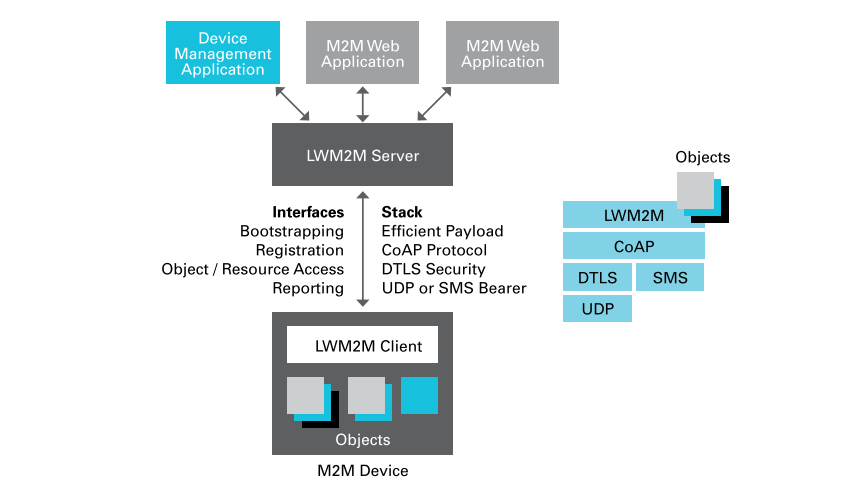
\includegraphics[width=\textwidth]{images/LWM2M-Architecture}
		\caption{LWM2M Architecture}
		\label{fig:LWM2MArchitecture}
	\end{center}
\end{figure}

The LWM2M Enabler defines the application layer communication protocol between Server and Client. It is separated into four logical interfaces, namely, Bootstrap, Device Discovery and Registration, Device Management and Service Enablement, and Information Reporting. Diagram showing interfaces and corresponding messages is illustrated in ~\ref{fig:LWM2MInterfaces}.

\begin{enumerate}
	\setlength{\itemsep}{1pt}
	\item Bootstrap: allows LWM2M Bootstrap server to manage keying, access control and to configure device for communication with the Server.
	\item Device Discovery and Registration: allows Server to discover devices and register their capabilities, e.g., which objects and how to access them does a device have.
	\item Device Management and Service Enablement: allows LWM2M Server to manage devices and provide M2M service by sending operations to devices and getting corresponding responses from them.
	\item Information Reporting: This is a core interface in LWM2M, which allows reporting of resource information. It can be triggered periodically, on events or on request.
\end{enumerate}

Communication model of LWM2M is based on CoAP methods similar to HTTP verbs GET, POST, PUT, DELETE to manipulate \emph{resources} on devices. Compared to HTTP, CoAP starts with only four bytes of overhead in binary encoded message and is easily translatable to HTTP. Unlike HTTP, CoAP messages are exchanged asynchronously between CoAP end-points over a datagram-oriented transport, in this case UDP.

In LWM2M Enabler, each individually addressable piece of information is called a Resource and groups of Resources are logically organized into Objects. For example, predefined object \emph{Location} contains all resources needed for locating the device. Full list of existing objects can be found at OMA registry \footnote{http://www.openmobilealliance.org/wp/OMNA/LwM2M/LwM2MRegistry.html}.

\begin{figure}[ht]
	\begin{center}
		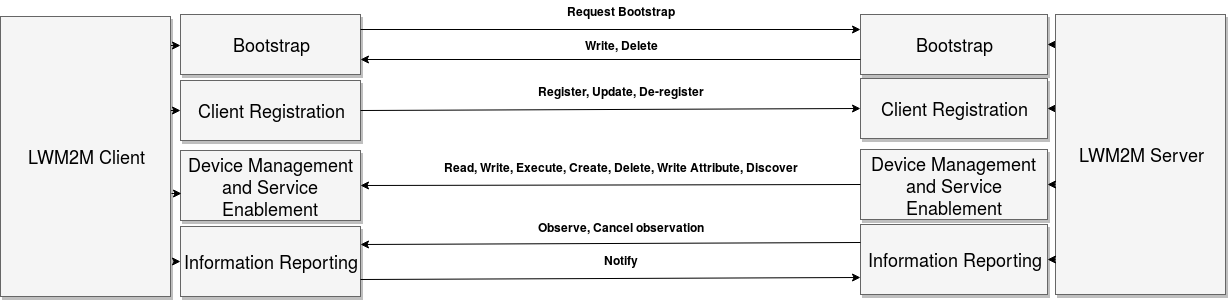
\includegraphics[width=\textwidth]{images/LWM2M-Interfaces}
		\caption{LWM2M Interfaces}
		\label{fig:LWM2MInterfaces}
	\end{center}
\end{figure}

\subsection{World-wide-web Consortium (W3C) - Web Of Things (WOT)}

Since there are many IOT platforms already existing, it is becoming a big problem for developers creating applications that span them. The solution W3C proposes aims to enable worldwide discovery and interoperability by exposing these platforms through the Web with a new class of webservers that support an open framework for the WOT as pictured on ~\ref{fig:WOTWebservers}. In other words, WOT aims to interconnect existing IOT platforms and complement available standards, to reduce cost and risk, and to boost market opportunities.

\begin{figure}[ht]
	\begin{center}
		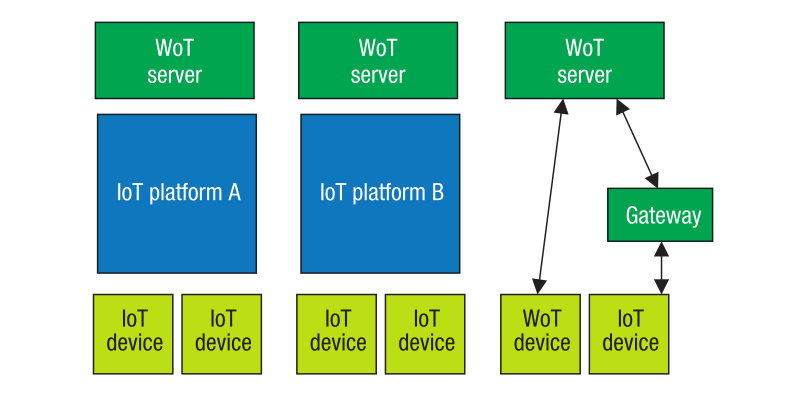
\includegraphics[width=\textwidth]{images/WOTWebservers}
		\caption{WOT framework that bridges the multiple existing IOT platforms}
		\label{fig:WOTWebservers}
	\end{center}
\end{figure}

In W3C WOT all things (devices) are modeled as events, properties and actions, while also possessing metadata describing location of the device, serial number and similar. Firstly, events represent notifications from device to server, such as "battery low" or "the door just opened". Secondly, properties represent information that can be checked through server, such as the temperature or the state of the light switch (on or off). Finally, actions represent commands to coming from server to the device, such as "move the crane from position x to position y" or "turn off". In order to retrieve matadata for things, WOT uses JavaScript Object Notation for Linked Data (JSON-LD).

Analogous to the role played by the Internet as an abstraction layer for networks and networking technologies, WOT describes an abstraction layer over heterogeneous IOT standards, communication patterns, protocols and data formats. This abstraction layer is pictured on figure ~\ref{fig:WOT}, where applications interact with software objects for things (devices, either virtual or physical). Webservers providing this abstraction can be placed on the edge of the network (or in the fog or cloud) to provide efficiency.

\begin{figure}[ht]
	\begin{center}
		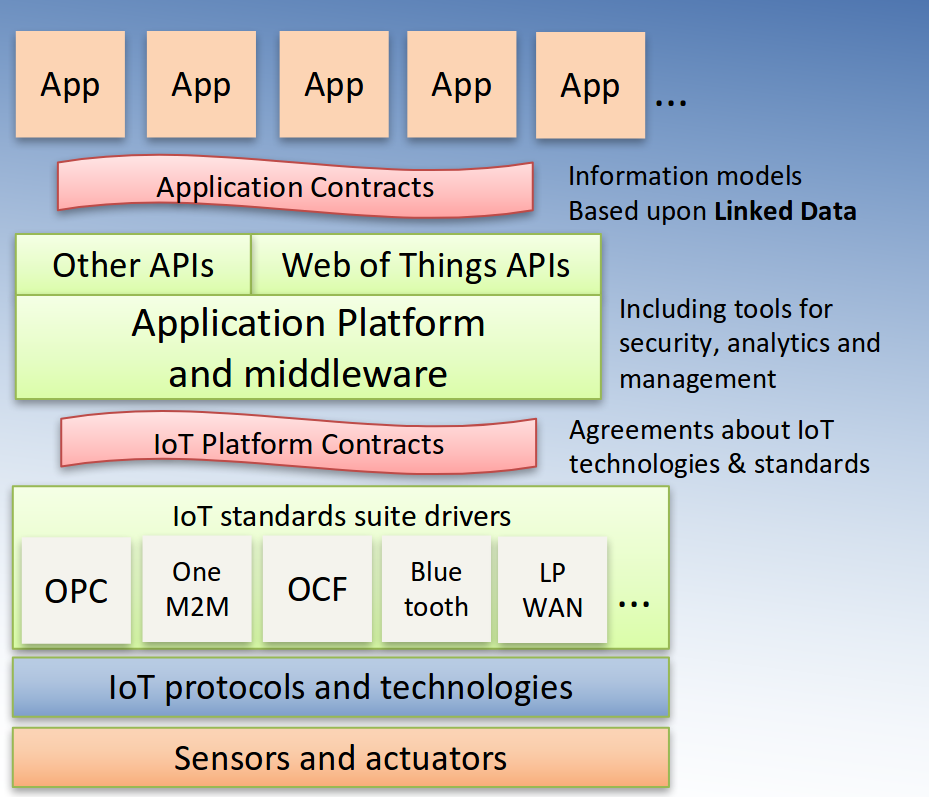
\includegraphics[width=\textwidth]{images/WOT}
		\caption{WOT abstraction layer}
		\label{fig:WOT}
	\end{center}
\end{figure}

Regarding security, WOT is building upon existing security standards such as IOT security foundation, and IOT platforms such as oneM2M (described in section ~\ref{section:Standardization}), claiming to provide end to end security. 

W3C WOT is a new standard, with the working group formed in the beginning of 2017. Since it is a new standard, their work has mostly been abstract, without any real implementations. It is relatively heavy weight compared to LWM2M standard, and focuses on providing a bridge between different platforms unlike LWM2M, that proposes a new solution not necessarily compatible with other existing solutions. Because the work on WOT is in a very early phase and reasons described above I have chosen to make use of LWM2M standard for this thesis.

\section{Policy Based Communications for 5G Mobile with Customer Edge Switching}
\label{CES}

Particularly interesting work by \cite{Kantola} proposes a policy based communication with built in security, while also addressing classical weaknesses of Internet, namely, address spoofing, unwanted traffic and DoS attacks. It is based on a principle that before establishing communication between two hosts (or networks) they need to negotiate interests, and only if they are matching communication is established. These interests are described with a policy.

This work proposes to replace Network Address Translator (NAT) from the edge of the network with their own Customer Edge Switch (CES) node. This node will act exactly like NAT if the sender, who is behind a CES node, is interacting with a receiver using legacy ip. On the other hand, if the situation is reversed CES node will act as a \emph{realm gateway}. Only if both actors are behind CES node it will act as a cooperative firewall negotiating interests of sender and receiver. Because of this, CES can be applied one network at a time making it suitable for IIOT purposes, where vertical fragmentation is a big issue.

Furthermore, CES allows efficient communication by dropping unwanted traffic at the edge and in that way reducing amount of traffic that passes trough network. Also, CES makes use of Domain Name Servers (DNS) to find receivers faster using Fully Qualified Domain Names (FQDN) and MS-ISDN numbers.

In essence, policy database holds all policies and can be accessed through API. Before communication is established, policies of both actors are checked and if they match communication is allowed. Example is shown on ~\ref{fig:PolicyBasedCommunicationExample}.

\begin{figure}[ht]
	\begin{center}
		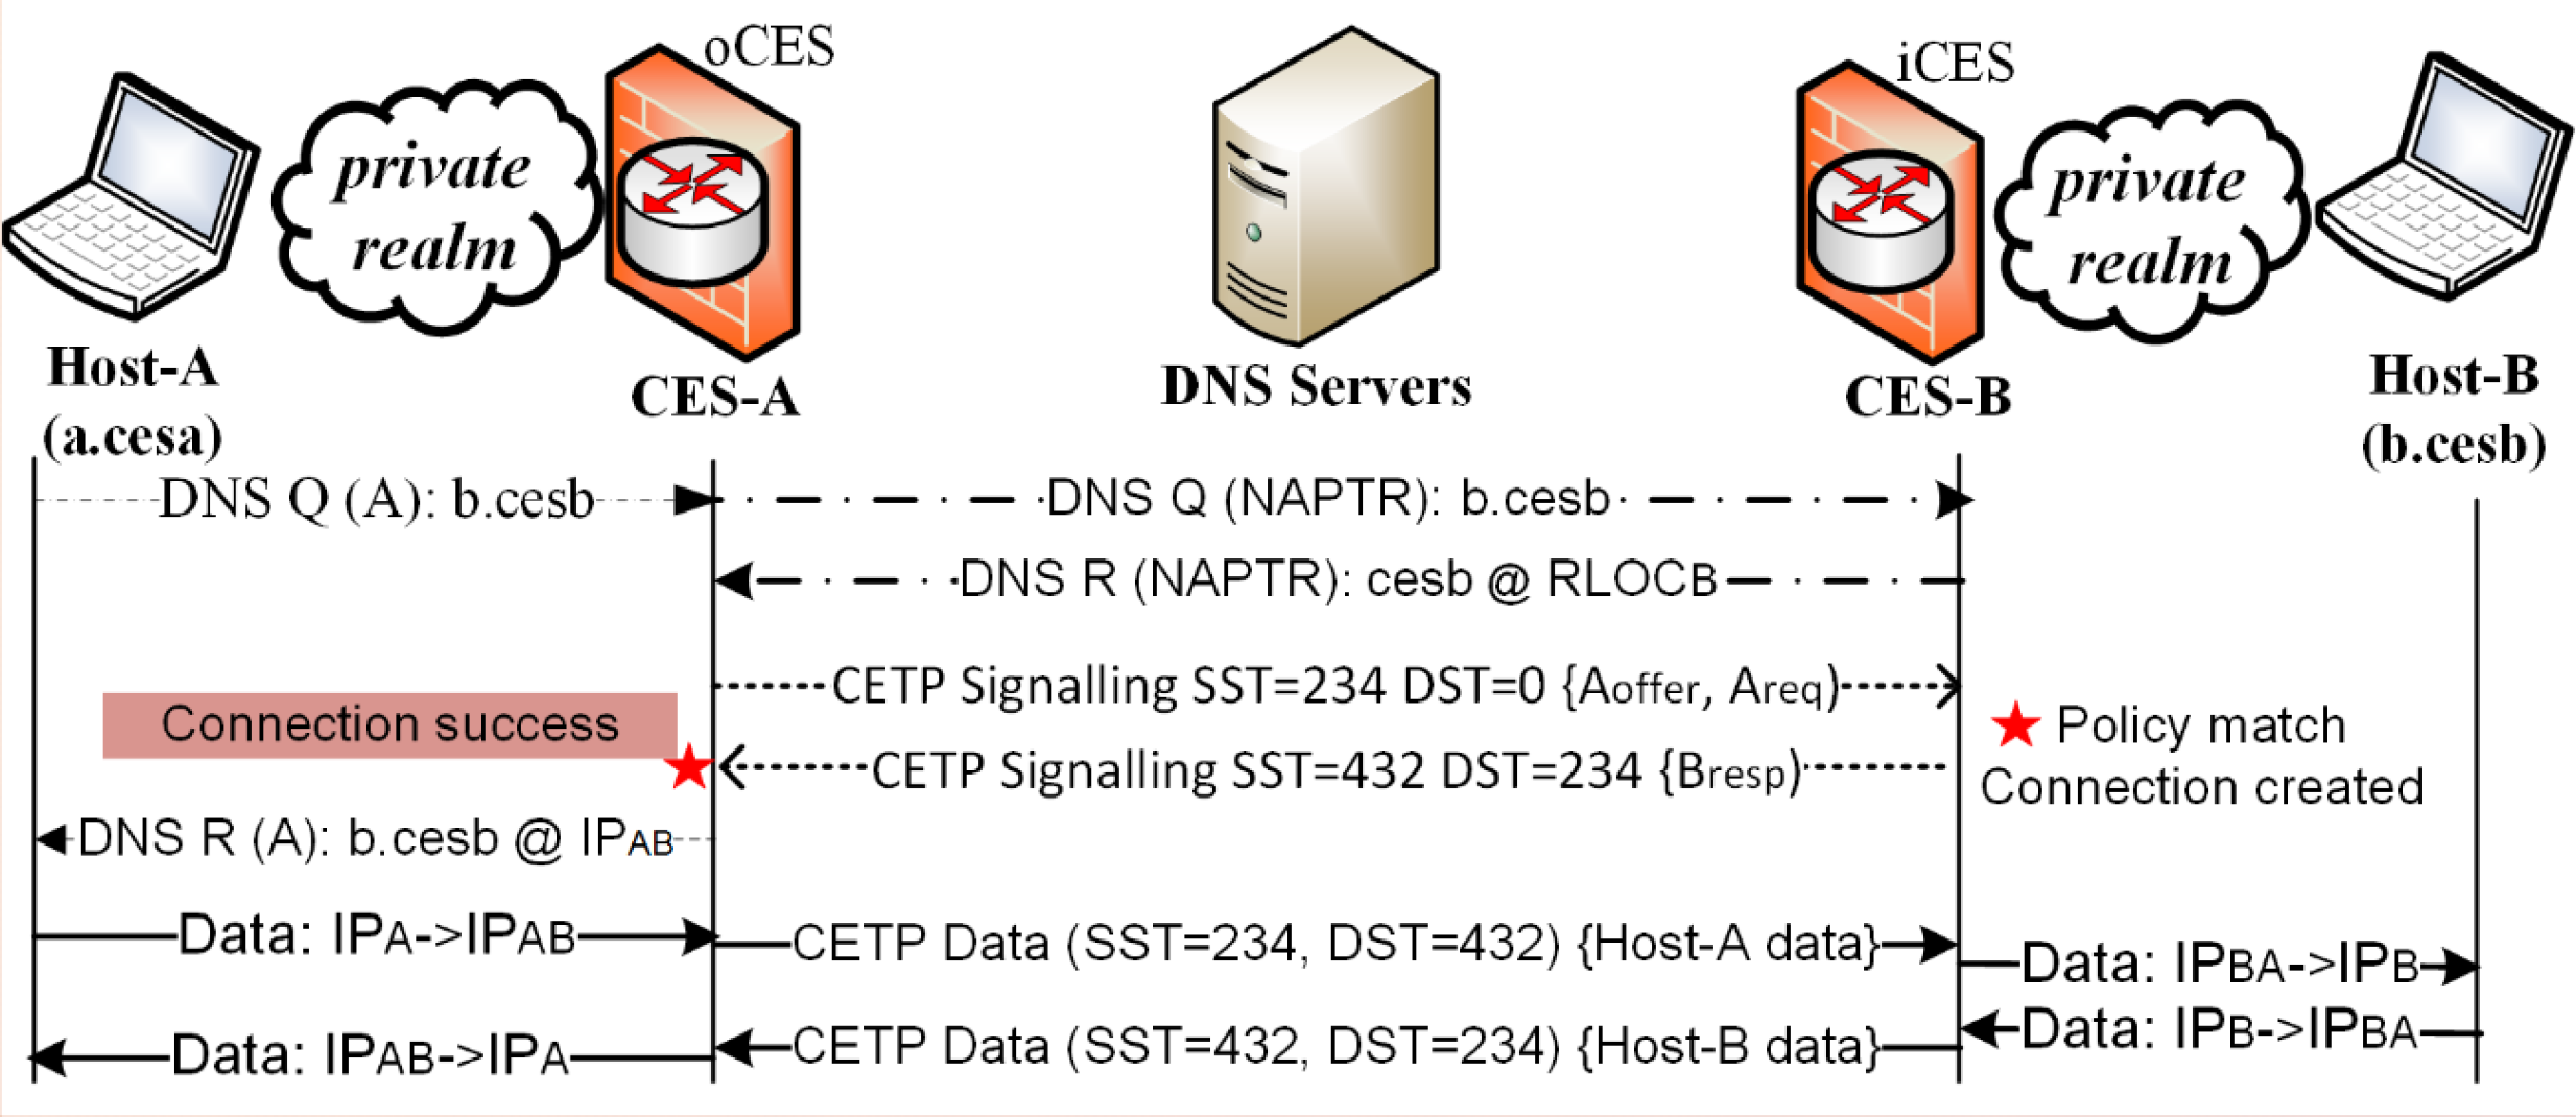
\includegraphics[width=\textwidth]{images/PolicyBasedCommunicationExample}
		\caption{CES communication example}
		\label{fig:PolicyBasedCommunicationExample}
	\end{center}
\end{figure}


\chapter{Environment}
\label{chapter:environment}

A problem instance is rarely totally independent of its environment.
Most often you need to describe the environment you work in, what
limits there are and so on. This is a good place to do that. First we
tell you about the LaTeX working environments and then is an example
from an thesis written some years ago.


\section{LaTeX working environments}
\label{sec:environments}

To create \LaTeX\ documents you need two things: a \LaTeX\ environment for
compiling your documents and a text editor for writing them.

\subsection{Environment}

Fortunately \LaTeX\ can nowadays be found for any (modern) computer
environment, be it Linux, Windows, or Macintosh.
For Linuxes (and other Unix clones) and Macs, I'd recommend \emph{TeX
Live}~\cite{TeXLive}, which is the current default \LaTeX\ distribution for
many Linux flavors such as Fedora, Debian, Ubuntu, and Gentoo.
TeX Live is the replacement for the older \emph{teTeX}, which is
no longer developed.

TeX Live works also for Windows machines (at least according to their web
site); however, I have used \emph{MiKTeX}~\cite{MiKTeX} and can recommend it
for Windows. 
MiKTeX has a nice package manager and automatically fetches missing packages
for you.

\subsection{Editor}

You can write \LaTeX\ documents with any text editor you like, but having
syntax coloring options and such really helps a lot.
My personal favourite for editing \LaTeX\ is the
\emph{TeXlipse}~\cite{TeXlipse} plugin for the Eclipse IDE~\cite{Eclipse}. 
Eclipse is an open-source integrated development environment (IDE) initially
created for writing Java code, but it currently has support for editing
languages such as C, C++, JavaScript, XML, HTML, and many more. 
The TeXlipse plugin allows you to edit and compile \LaTeX\ documents directly
in Eclipse, and compilation errors and warnings are shown in the Eclipse
\emph{Problems} dialog so that you can locate and fix the issues easily.
The plugin also supports reference traversal so that you can locate the source
line where a label or a citation is defined.

Eclipse is an entire development environment, so it may feel a bit heavy-weight
for editing a document. 
If you are looking for a more light-weight option, check out TeXworks. 
TeXworks is a \LaTeX\ editor that is packaged with the newer MiKTeX
distributions, and it can be acquired from \url{http://www.tug.org/texworks/}.

And if you are attached to your \emph{emacs} or \emph{vim} editor, you
can of course edit your \LaTeX\ documents with them. 
Emacs at least has syntax coloring and you can compile your document with a key
binding, so this may be a good option if you prefer working with the standard
Linux text editors.

\section{Graphics}

When you use \texttt{pdflatex} to render your thesis, you can include PDF images
directly, as shown by Figure~\ref{fig:indica_model} below.

\begin{figure}[ht]
  \begin{center}
    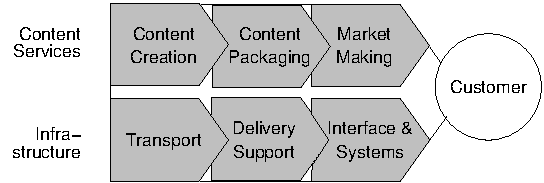
\includegraphics[width=\textwidth]{images/indica_model.pdf}
    \caption{The INDICA two-layered value chain model.}
    \label{fig:indica_model}
  \end{center}
\end{figure}

You can also include JPEG or PNG files, as shown by Figure~\ref{fig:eeyore}.

\begin{figure}[ht]
  \begin{center}
    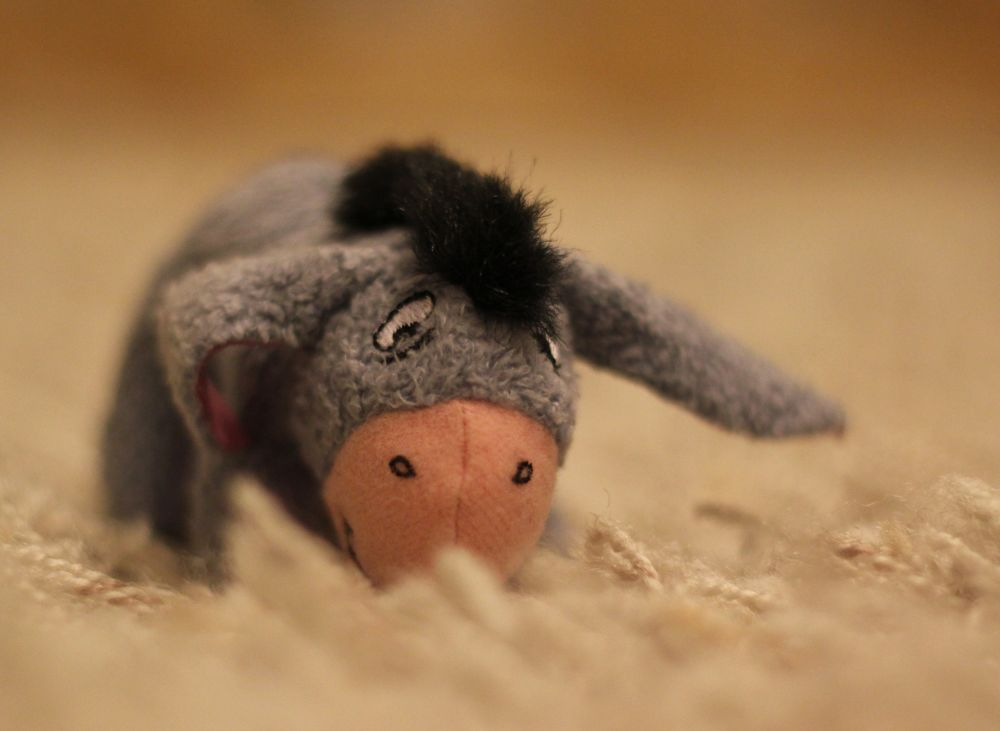
\includegraphics[width=9cm]{images/ihaa.jpg}
    \caption{Eeyore, or Ihaa, a very sad donkey.}
    \label{fig:eeyore}
  \end{center}
\end{figure}

You can create PDF files out of practically anything. 
In Windows, you can download PrimoPDF or CutePDF (or some such) and install a
printing driver so that you can print directly to PDF files from any
application. There are also tools that allow you to upload documents in common
file formats and convert them to the PDF format.
If you have PS or EPS files, you can use the tools \texttt{ps2pdf} or
\texttt{epspdf} to convert your PS and EPS files to PDF\@.

% Comment: If your sentence ends in a capital letter, like here, you should
% write \@ before the period; otherwise LaTeX will assume that this is not
% really an end of the sentence and will not put a large enough space after the
% period. That is, LaTeX assumes that you are (for example), enumerating using
% capital roman numerals, like I. do something, II. do something else. In this
% case, the periods do not end the sentence.

% Similarly, if you do need a normal space after a period (instead of
% the longer sentence separator), use \  (backslash and space) after the
% period. Like so: a.\ first item, b.\ second item.

Furthermore, most newer editor programs allow you to save directly to the PDF
format. For vector editing, you could try Inkscape, which is a new open source
WYSIWYG vector editor that allows you to save directly to PDF\@. 
For graphs, either export/print your graphs from OpenOffice Calc/Microsoft
Excel to PDF format, and then add them; or use \texttt{gnuplot}, which can
create PDF files directly (at least the new versions can).
The terminal type is \emph{pdf}, so the first line of your plot file should be
something like \texttt{set term pdf \ldots}.

To get the most professional-looking graphics, you can encode them using the
TikZ package (TikZ is a frontend for the PGF graphics formatting system).
You can create practically any kind of technical images with TikZ, but it has a
rather steep learning curve. Locate the manual (\texttt{pgfmanual.pdf}) from
your \LaTeX\ distribution and check it out. An example of TikZ-generated
graphics is shown in Figure~\ref{fig:page-merge}.

\begin{figure}[ht]
  \begin{center}
    \newcommand*{\actver}{\smash{\ensuremath{v_{\text{\textit{active}}}}}}

\tikzstyle{lbl}=[font=\scriptsize,midway,sloped]
\tikzstyle{opendash}=[densely dotted,thick] 
\tikzstyle{opendeco}=[decoration={zigzag,amplitude=0.1em,segment length=0.6em}]
\tikzstyle{actverline}=[dashed]
\tikzstyle{entryline}=[densely dotted]
\tikzstyle{area}=[ellipse,draw,dashed]
\tikzstyle{liveentry}=[entryline,postaction={%
  decorate,%
  decoration={%
    markings,%
    mark=at position .5pt with{\arrowreversed[line width=.35pt]{|}};,
    mark=at position 1 with{%
      \arrow[line width=.8pt]{stealth}};%
  }%
}]
\tikzstyle{deadentry}=[entryline,postaction={%
  decorate,%
  decoration={%
    markings,%
    mark=at position .5pt with{\arrowreversed[line width=.35pt]{|}};,
    mark=at position 1 with{%
      \arrow[line width=.8pt]{stealth}};%
%      \arrow[line width=.35pt,black,fill=white]{*}};% 
  }%
}]
\tikzstyle{pageborder}=[thick]
\tikzstyle{pagename}=[anchor=center,text=black!50,font=\huge]
\newlength{\spexx}
\setlength{\spexx}{1.2cm}
\newlength{\spexy}
\setlength{\spexy}{.5cm}

\subfigure[Before]{
\begin{tikzpicture}[x=\spexx,y=\spexy,%
  every pin edge/.style={draw,dotted},%
  pin distance=.5\spexx]
  \small
  \coordinate (lo) at (0,-5);
  \coordinate (o) at (0,0);
  \coordinate (hi) at (0,7);
  \coordinate (loact) at (3,-5);
  \coordinate (oact) at (3,0);
  \coordinate (hiact) at (3,7);
  \coordinate (loinf) at (4,-5);
  \coordinate (oinf) at (4,0);
  \coordinate (hiinf) at (4,7);
  
  \draw[->] (lo) -- node[below,lbl] {Versions} ($(loinf) + (1em,0)$);
  \draw[->] (lo) -- node[above,lbl] {Keys} ($(hi) + (0,1em)$);

  \draw[pageborder] (lo) -- (o) -- (hi);
  \draw[pageborder] (lo) -- (loinf);
  \draw[pageborder] (hi) -- (hiinf);
  \draw[pageborder] (o) -- (oinf);

  \draw[opendash] decorate [opendeco] { (loinf) -- (oinf) };
  \draw[opendash] decorate [opendeco] { (oinf) -- (hiinf) };

  \node[pagename] at (2,3.5) {$p$};
  \node[pagename] at (2,-2.5) {$s$};

  \draw[actverline] ($(loact) + (0,-1em)$) node[below=.4em] {\actver} --
    ($(hiact) + (0,1em)$);

  % Page p contents
  \draw[deadentry] (0,6) -- (1,6);
  \draw[deadentry] (1,6) -- (2,6);
  \draw[deadentry] (2,6) -- (3,6);
  \draw[liveentry] (0,5) -- (4,5);
  \draw[deadentry] (0,4) -- (2,4);
  \draw[deadentry] (1,3) -- (3,3);
  \draw[deadentry] (0,2) -- (1,2);
  \draw[deadentry] (2,2) -- (3,2);
  \draw[deadentry] (0,1) -- (2,1);
  \draw[deadentry] (2,1) -- (3,1);

  % Page s contents
  \draw[liveentry] (0,-1) -- (4,-1);
  \draw[deadentry] (0,-2) -- (2,-2);
  \draw[deadentry] (0,-3) -- (3,-3);
  \draw[liveentry] (3,-4) -- (4,-4);

  \node[area,minimum width=4.5\spexx,minimum height=.6\spexy,pin=178:{$1$}]
    at (2,5) {};
  \node[area,minimum width=4.5\spexx,minimum height=.6\spexy,pin=182:{$2$}]
    at (2,-1) {};
  \node[area,minimum width=1.5\spexx,minimum height=.6\spexy,pin=330:{$3$}]
    at (3.5,-4) {};

\end{tikzpicture}}
\subfigure[After]{
\begin{tikzpicture}[x=\spexx,y=\spexy,%
  every pin edge/.style={draw,dotted},%
  pin distance=.5\spexx]
  \small
  \coordinate (lo) at (0,-5);
  \coordinate (o) at (0,0);
  \coordinate (hi) at (0,7);
  \coordinate (loact) at (3,-5);
  \coordinate (oact) at (3,0);
  \coordinate (hiact) at (3,7);
  \coordinate (loinf) at (4,-5);
  \coordinate (oinf) at (4,0);
  \coordinate (hiinf) at (4,7);

  \draw[->] (lo) -- node[lbl,below] {Versions} ($(loinf) + (1em,0)$);
  \draw[->] (lo) -- node[lbl,above] {Keys} ($(hi) + (0,1em)$);

  \draw[pageborder] (lo) -- (o) -- (hi);
  \draw[pageborder] (lo) -- (loinf);
  \draw[pageborder] (hi) -- (hiinf);
  \draw[pageborder] (o) -- (oact);

  \draw[opendash] decorate [opendeco] { (loinf) -- (oinf) };
  \draw[opendash] decorate [opendeco] { (oinf) -- (hiinf) };

  \node[pagename] at (1.5,3.5) {$p$};
  \node[pagename] at (1.5,-2.5) {$s$};
  \node[pagename] at (3.5,1) {$p'$};

  \draw[actverline] ($(loact) + (0,-1em)$) node[below=.4em] {\actver} -- (loact);
  \draw[pageborder] (loact) -- (hiact);
  \draw[actverline] (hiact) -- ($(hiact) + (0,1em)$);

  % Page p contents
  \draw[deadentry] (0,6) -- (1,6);
  \draw[deadentry] (1,6) -- (2,6);
  \draw[deadentry] (2,6) -- (3,6);
  \draw[deadentry] (0,5) -- (3,5);
  \draw[deadentry] (0,4) -- (2,4);
  \draw[deadentry] (1,3) -- (3,3);
  \draw[deadentry] (0,2) -- (1,2);
  \draw[deadentry] (2,2) -- (3,2);
  \draw[deadentry] (0,1) -- (2,1);
  \draw[deadentry] (2,1) -- (3,1);

  % Page s contents
  \draw[deadentry] (0,-1) -- (3,-1);
  \draw[deadentry] (0,-2) -- (2,-2);
  \draw[deadentry] (0,-3) -- (3,-3);

  % Page p' contents
  \draw[liveentry] (3,5) -- (4,5);
  \draw[liveentry] (3,-1) -- (4,-1);
  \draw[liveentry] (3,-4) -- (4,-4);

  \node[area,minimum width=1.5\spexx,minimum height=.6\spexy,pin=10:{$1$}]
    at (3.5,5) {};
  \node[area,minimum width=1.5\spexx,minimum height=.6\spexy,pin=3:{$2$}]
    at (3.5,-1) {};
  \node[area,minimum width=1.5\spexx,minimum height=.6\spexy,pin=330:{$3$}]
    at (3.5,-4) {};
\end{tikzpicture}}

    \caption{Example of a multiversion database page merge. This figure has
    been taken from the PhD thesis of Haapasalo~\cite{HaapasaloThesis}.}
    \label{fig:page-merge}
  \end{center}
\end{figure}

Another example of graphics created with TikZ is shown in
Figure~\ref{fig:tikz-examples}. 
These show how graphs can be drawn and labeled. 
You can consult the example images and the PGF manual for more examples of what
kinds figures you can draw with TikZ. 

% These definitions are only used in the example images; you will not 
% need them for your thesis...
\newlength{\graphdotsize}
\setlength{\graphdotsize}{1.7pt}
\newlength{\graphgridsize}
\setlength{\graphgridsize}{1.2em}
\begin{figure}[ht]
\begin{center}
\subfigure[Examples of obstruction graphs for the Ferry Problem]{
  \newlength{\oggs}
\setlength{\oggs}{1.2\graphgridsize}
\begin{tikzpicture}[x=\oggs,y=\oggs,every pin edge/.style={draw,dotted},pin distance=0.5\oggs,area/.style={ellipse,draw,dashed}] 

% The graph (0,0,5,0)
% o = origo
\coordinate (o) at (0,0);
\coordinate[left=1 of o,pin=100:$q_1$] (q1);
\coordinate[right=1 of o,pin=80:$q_2$] (q2);
\fill[black] (q1) circle (\graphdotsize);
\fill[black] (q2) circle (\graphdotsize);
\foreach \d in {-2, -1, ..., 2} {
  \coordinate (tmp) at ($(o) + (0,\d)$);
  \draw (q1) -- (tmp);
  \draw (q2) -- (tmp);
  \fill[black] (tmp) circle (\graphdotsize);
}
\node[area,minimum height=5.3\oggs,minimum width=0.8\oggs,pin=94:$X_3$] at (o) {};  

% The graph (1,0,3,0)
\coordinate[right=5 of o] (o);
\coordinate[left=1 of o,pin=260:$q_1$] (q1);
\coordinate[left=2 of o] (q1v);
\coordinate[right=1 of o,pin=280:$q_2$] (q2);
\fill[black] (q1) circle (\graphdotsize);
\fill[black] (q2) circle (\graphdotsize);
\fill[black] (q1v) circle (\graphdotsize);
\draw (q1) -- (q1v);
\foreach \d in {-1, 0, 1} {
  \coordinate (tmp) at ($(o) + (0,\d)$);
  \draw (q1) -- (tmp);
  \draw (q2) -- (tmp);
  \fill[black] (tmp) circle (\graphdotsize);
}
\node[area,minimum height=3.3\oggs,minimum width=0.8\oggs,pin=266:$X_3$] at (o) {};  
\node[area,minimum height=0.8\oggs,minimum width=0.8\oggs,pin=260:$X_1$] at (q1v) {};  


% The graph (0,1,3,0)
\coordinate[right=4 of o] (o);
\coordinate[left=1 of o,pin=100:$q_1$] (q1);
\coordinate[right=1 of o,pin=80:$q_2$] (q2);
\coordinate[right=2 of o] (q2v);
\fill[black] (q1) circle (\graphdotsize);
\fill[black] (q2) circle (\graphdotsize);
\fill[black] (q2v) circle (\graphdotsize);
\draw (q2) -- (q2v);
\foreach \d in {-1, 0, 1} {
  \coordinate (tmp) at ($(o) + (0,\d)$);
  \draw (q1) -- (tmp);
  \draw (q2) -- (tmp);
  \fill[black] (tmp) circle (\graphdotsize);
}
\node[area,minimum height=3.3\oggs,minimum width=0.8\oggs,pin=94:$X_3$] at (o) {};  
\node[area,minimum height=0.8\oggs,minimum width=0.8\oggs,pin=80:$X_2$] at (q2v) {};  

% The graph (0,0,3,1)
\coordinate[right=5 of o] (o);
\coordinate[left=1 of o,pin=260:$q_1$] (q1);
\coordinate[right=1 of o,pin=290:$q_2$] (q2);
\fill[black] (q1) circle (\graphdotsize);
\fill[black] (q2) circle (\graphdotsize);
\draw (q1) -- (q2);
\foreach \d in {-1, 1, 2} {
  \coordinate (tmp) at ($(o) + (0,\d)$);
  \draw (q1) -- (tmp);
  \draw (q2) -- (tmp);
  \fill[black] (tmp) circle (\graphdotsize);
}
\node[area,minimum height=4.3\oggs,minimum width=0.8\oggs,pin=266:$X_3$] at ($(o) + (0,0.5)$) {};  

\end{tikzpicture}

}
\subfigure[Examples of star graphs]{
  \begin{tikzpicture}[x=\graphgridsize,y=\graphgridsize] 

\coordinate (o) at (0,0);
\fill[black] (o) circle (\graphdotsize);
\foreach \d in {0, 90, ..., 270} {
  \coordinate (tmp) at ($(o) + (\d:1.5)$);
  \draw (o) -- (tmp);
  \fill[black] (tmp) circle (\graphdotsize);
}

\coordinate[right=4 of o] (o);
\coordinate (o1) at ($(o) + (0:0.3)$);
\coordinate (o2) at ($(o) + (180:0.3)$);
\fill[black] (o1) circle (\graphdotsize);
\fill[black] (o2) circle (\graphdotsize);
\draw (o1) -- (o2);
\foreach \d in {45, 135, 270} {
  \coordinate (tmp\d) at ($(o) + (\d:1.5)$);
  \draw (o2) -- (tmp\d);
  \fill[black] (tmp\d) circle (\graphdotsize);
}
\draw (o1) -- (tmp45);


\coordinate[right=4 of o] (o);
\coordinate (o1) at ($(o) + (0:0.3)$);
\coordinate (o2) at ($(o) + (180:0.3)$);
\fill[black] (o1) circle (\graphdotsize);
\fill[black] (o2) circle (\graphdotsize);
\draw (o1) -- (o2);
\foreach \d in {45, 135, 270} {
  \coordinate (tmp\d) at ($(o) + (\d:1.5)$);
  \draw (o2) -- (tmp\d);
  \fill[black] (tmp\d) circle (\graphdotsize);
}
\draw (o1) -- (tmp45);
\draw (o1) -- (tmp135);


\coordinate[right=4 of o] (o);
\coordinate (o1) at ($(o) + (0:0.3)$);
\coordinate (o2) at ($(o) + (180:0.3)$);
\fill[black] (o1) circle (\graphdotsize);
\fill[black] (o2) circle (\graphdotsize);
\draw (o1) -- (o2);
\foreach \d in {45, 135, 270} {
  \coordinate (tmp\d) at ($(o) + (\d:1.5)$);
  \draw (o1) -- (tmp\d);
  \draw (o2) -- (tmp\d);
  \fill[black] (tmp\d) circle (\graphdotsize);
}


\coordinate[right=3.5 of o] (o);
\coordinate (o1) at ($(o) + (90:0.3)$);
\coordinate (o2) at ($(o) + (210:0.5)$);
\coordinate (o3) at ($(o) + (330:0.5)$);
\fill[black] (o1) circle (\graphdotsize);
\fill[black] (o2) circle (\graphdotsize);
\fill[black] (o3) circle (\graphdotsize);
\draw (o1) -- (o2);
\draw (o1) -- (o3);
\draw (o2) -- (o3);
\foreach \d in {90, 270} {
  \coordinate (tmp\d) at ($(o) + (\d:1.5)$);
  \draw (o2) -- (tmp\d);
  \draw (o3) -- (tmp\d);
  \fill[black] (tmp\d) circle (\graphdotsize);
}
\draw (o1) -- (tmp90);


\coordinate[right=3 of o] (o);
\coordinate (o1) at ($(o) + (90:0.3)$);
\coordinate (o2) at ($(o) + (210:0.5)$);
\coordinate (o3) at ($(o) + (330:0.5)$);
\fill[black] (o1) circle (\graphdotsize);
\fill[black] (o2) circle (\graphdotsize);
\fill[black] (o3) circle (\graphdotsize);
\draw (o1) -- (o2);
\draw (o1) -- (o3);
\draw (o2) -- (o3);
\foreach \d in {90, 270} {
  \coordinate (tmp\d) at ($(o) + (\d:1.5)$);
  \draw (o2) -- (tmp\d);
  \draw (o3) -- (tmp\d);
  \fill[black] (tmp\d) circle (\graphdotsize);
}
\draw (o1) -- (tmp90);
\draw (o1) -- (tmp270);



\coordinate[right=3.5 of o] (o);
\coordinate (o1) at ($(o) + (18:1.3)$);
\coordinate (o2) at ($(o) + (90:1.3)$);
\coordinate (o3) at ($(o) + (162:1.3)$);
\coordinate (o4) at ($(o) + (234:1.3)$);
\coordinate (o5) at ($(o) + (306:1.3)$);
\foreach \d in {1, 2, ..., 5} {
  \fill[black] (o\d) circle (\graphdotsize);
}
\draw (o1) -- (o2);
\draw (o1) -- (o3);
\draw (o1) -- (o4);
\draw (o1) -- (o5);
\draw (o2) -- (o3);
\draw (o2) -- (o4);
\draw (o2) -- (o5);
\draw (o3) -- (o4);
\draw (o3) -- (o5);
\draw (o4) -- (o5);

\end{tikzpicture}

}
\caption{Examples of graphs draw with TikZ. These figures have been taken from a
course report for the graph theory course~\cite{FerryProblem}.}
\label{fig:tikz-examples}
\end{center}
\end{figure}



\chapter{Methods}
\label{chapter:methods}

You have now stated your problem, and you are ready to do something
about it!  \emph{How} are you going to do that? What methods do you
use?  You also need to review existing literature to justify your
choices, meaning that why you have chosen the method to be applied in
your work.

% An example of a traditional LaTeX table
% ------------------------------------------------------------------
% A note on underfull/overfull table cells and tables:
% ------------------------------------------------------------------
% In professional typography, the width of the text in a page is always a lot
% less than the width of the page. If you are accustomed to the (too wide) text
% areas used in Microsoft Word's standard documents, the width of the text in
% this thesis layout may suprise you. However, text in a book needs wide
% margins. Narrow text is easier to read and looks nicer. Longer lines are 
% hard to read, because the start of the next line is harder to locate when
% moving from line to the next. 
% However, tables that are in the middle of the text often would require a wider
% area. By default, LaTeX will complain if you create too wide tables with
% ``overfull'' error messages, and the table will not be positioned properly
% (not centered). If at all possible, try to make the table narrow enough so
% that it fits to the same space as the text (total width = \textwidth).
% If you do need more space, you can either
% 1) ignore the LaTeX warnings 
% 2) use the textpos-package to manually position the table (read the package
%    documentation)
% 3) if you have the table as a PDF document (of correct size, A4), you can use
%    the pdfpages package to include the page. This overrides the margin
%    settings for this page and LaTeX will not complain.
% ------------------------------------------------------------------
% Another note:
% ------------------------------------------------------------------
% If your table fits to \textwidth, but the cells are so narrow that the text
% in p{..}-formatted cells does not flow nicely (you get underfull warnings 
% because LaTeX tries to justify the text in the cells) you can manually set
% the text to unjustified by using the \raggedright command for each cell 
% that you do not want to be justified (see the example below). \raggedleft 
% is also possible, of course...
% ------------------------------------------------------------------
% If you need to have linefeeds (\\) inside a cell, you must create a new
% paragraph-formatting environment inside the cell. Most common ones are 
% the minipage-environment and the \parbox command (see LaTeX documentation
% for details; or just google for ``LaTeX minipage'' and ``LaTeX parbox'').
\begin{table}
\begin{tabular}{|p{2cm}|p{3.8cm}|p{4.5cm}|p{1.1cm}|} 
% Alignment of sells: l=left, c=center, r=right. 
% If you want wrapping lines, use p{width} exact cell widths.
% If you want vertical lines between columns, write | above between the letters
% Horizontal lines are generated with the \hline command:
\hline % The line on top of the table
\textbf{Code} & \textbf{Name} & \textbf{Methods} & \textbf{Area} \\ 
\hline 
% Place a & between the columns
% In the end of the line, use two backslashes \\ to break the line,
% then place a \hline to make a horizontal line below the row 
T-110.6130 & Systems Engineering for Data Communications
    Software & \raggedright Computer simulations, mathematical modeling,
  experimental research, data analysis, and network service business
  research methods, (agile method) & T-110 \\ 
\hline
\multicolumn{2}{|p{6.25cm}|}{Mat-2.3170 Simulation (here is an example of
 multicolumn for tables)}& Details of how to build simulations & T-110 \\
% The multicolumn command takes the following 3 arguments: 
% the number of cells to merge, the cell formatting for the new cell, and the
% contents of the cell
\hline
S-38.3184 & Network Traffic Measurements and Analysis 
& \raggedright How to measure and analyse network
  traffic & T-110 \\ \hline
\end{tabular} % for really simple tables, you can just use tabular
% You can place the caption either below (like here) or above the table
\caption{Research methodology courses}
% Place the label just after the caption to make the link work
\label{table:courses}
\end{table} % table makes a floating object with a title

If you have not yet done any (real) metholodogical courses (but chosen
introduction courses of different areas that are listed in the
methodological courses list), now is the time to do so or at least
check through material of suitable methodological courses. Good
methodologial courses that consentrates especially to methods are
presented in Table~\ref{table:courses}. Remember to explain the
content of the tables (as with figures). In the table, the last column
gives the research area where the methods are often used. Here we used
table to give an example of tables. Abbreviations and Acronyms is also
a long table. The difference is that longtables can continue to next
page.


 
\chapter{Implementation}
\label{chapter:implementation}

You have now explained how you are going to tackle your problem. 
Go do that now! Come back when the problem is solved!

Now, how did you solve the problem? 
Explain how you implemented your solution, be it a software component, a
custom-made FPGA, a fried jelly bean, or whatever.
Describe the problems you encountered with your implementation work.



\chapter{Evaluation}
\label{chapter:evaluation}

You have done your work, but that's\footnote{By the way, do \emph{not} use
shorthands like this in your text! It is not professional! Always write out all
the words: ``that is''.} not enough. 

You also need to evaluate how well your implementation works.  The
nature of the evaluation depends on your problem, your method, and
your implementation that are all described in the thesis before this
chapter.  If you have created a program for exact-text matching, then
you measure how long it takes for your implementation to search for
different patterns, and compare it against the implementation that was
used before.  If you have designed a process for managing software
projects, you perhaps interview people working with a waterfall-style
management process, have them adapt your management process, and
interview them again after they have worked with your process for some
time. See what's changed.

The important thing is that you can evaluate your success somehow.
Remember that you do not have to succeed in making something spectacular; a
total implementation failure may still give grounds for a very good master's
thesis---if you can analyze what went wrong and what should have been done.

 

 
\chapter{Discussion}
\label{chapter:discussion}

At this point, you will have some insightful thoughts on your implementation
and you may have ideas on what could be done in the future. 
This chapter is a good place to discuss your thesis as a whole and to show your
professor that you have really understood some non-trivial aspects of the
methods you used\ldots


 
\chapter{Conclusions}
\label{chapter:conclusions}

Time to wrap it up! 
Write down the most important findings from your work. 
Like the introduction, this chapter is not very long.
Two to four pages might be a good limit. 



% Load the bibliographic references
% ------------------------------------------------------------------
% You can use several .bib files:
% \bibliography{thesis_sources,ietf_sources}
\bibliography{sources}


% Appendices go here
% ------------------------------------------------------------------
% If you do not have appendices, comment out the following lines
\appendix
\chapter{First appendix}
\label{chapter:first-appendix}

This is the first appendix. You could put some test images or verbose data in an
appendix, if there is too much data to fit in the actual text nicely.

For now, the Aalto logo variants are shown in Figure~\ref{fig:aaltologo}.

\begin{figure}
\begin{center}
\subfigure[In English]{
\includegraphics[width=.8\textwidth]{images/aalto-logo-en}}
\subfigure[Suomeksi]{
\includegraphics[width=.8\textwidth]{images/aalto-logo-fi}}
\subfigure[På svenska]{
\includegraphics[width=.8\textwidth]{images/aalto-logo-se}}
\caption{Aalto logo variants}
\label{fig:aaltologo}
\end{center}
\end{figure}

% End of document!
% ------------------------------------------------------------------
% The LastPage package automatically places a label on the last page.
% That works better than placing a label here manually, because the
% label might not go to the actual last page, if LaTeX needs to place
% floats (that is, figures, tables, and such) to the end of the 
% document.
\end{document}
